\chapter{Волновые функции, матрицы плотности и локальность}

\lectureoverview{Теорема Белла откладывается по одной существенной причине: прежде чем спрашивать, что именно запрещает Белл, мы должны точно сказать, что такое запутанность. Бипартитное состояние является запутанным, когда его нельзя факторизовать в одно состояние для Алисы и одно для Боба. Волновые функции делают этот критерий конкретным, корреляции выявляют его следствия, а синглет дает решающий пример. Тогда редуцированная матрица плотности становится полным локальным описанием одной части запутанного целого. Имея этот аппарат, мы видим, что измерение выступает как запутывающее взаимодействие, границу система--наблюдатель можно перемещать без изменения предсказаний, и кажущееся напряжение между запутанностью и локальностью можно сформулировать точно: удаленные выборы изменяют условные корреляции, но не безусловную статистику, доступную для передачи сигналов.}

\section{Что на самом деле означает запутанность}

Заманчиво сразу перейти к теореме Белла. Теорема прекрасна, но ее значение нельзя отделить от структуры, которую она проверяет. Поэтому более насущный вопрос сейчас еще не в том, нарушает ли квантовая механика неравенство Белла, а в том, что запутанное состояние говорит о составной системе.

Расхожая фраза состоит в том, что две запутанные системы \emph{имеют общее состояние}. Эта фраза ничего не различает. У любой составной системы есть состояние, запутана она или нет. Существенное различие — в факторизации. Если \(A\) и \(B\) имеют гильбертовы пространства \(\mathcal H_A\) и \(\mathcal H_B\), то состояние пары принадлежит
\begin{equation}
\mathcal H_{AB}=\mathcal H_A\otimes\mathcal H_B.
\end{equation}
Чистое состояние является состоянием-произведением, если его можно записать как
\begin{equation}
\ket{\Psi}_{AB}=\ket{\psi}_A\otimes\ket{\phi}_B.
\label{eq:l7-product-state}
\end{equation}
Если такой пары множителей не существует, \(\ket{\Psi}_{AB}\) запутано.

\begin{classroomqa}
\audiencequestion{Означает ли запутанность просто то, что обе системы описываются одним вектором состояния?}
\lecturerresponse{Нет. Состояние-произведение тоже принадлежит гильбертову пространству всей пары. Запутанность — это более сильное, не зависящее от базиса утверждение: вектор целого нельзя записать в виде произведения одного вектора для Алисы и одного для Боба.}
\end{classroomqa}

\begin{classroomqa}
\audiencequestion{Может ли удачно выбранная замена базиса превратить запутанное состояние в состояние-произведение?}
\lecturerresponse{Не может, если замена базиса локальна, то есть представляет собой одну замену базиса для Алисы и другую для Боба. Локальные замены базиса изменяют координаты каждого множителя, но не изменяют того, факторизуется ли состояние. Совершенно произвольный базис совместного гильбертова пространства может скрыть структуру тензорного произведения, но он не меняет, какие физические степени свободы принадлежат Алисе и Бобу.}
\end{classroomqa}

\section{Волновые функции как координаты в гильбертовом пространстве}

Слово \emph{волновая функция} несет исторические ассоциации, которые не входят в его математическое определение. Волновая функция — это координатное представление вектора состояния в выбранном базисе. Пусть полный набор коммутирующих наблюдаемых имеет общие собственные векторы
\begin{equation}
\ket{a,b,c,\ldots}.
\end{equation}
Метки должны быть полными: взятые вместе, они различают каждый вектор базиса. Тогда
\begin{align}
\ket{\Psi}
&=\sum_{a,b,c,\ldots}
\ket{a,b,c,\ldots}
\braket{a,b,c,\ldots}{\Psi} \\
&=\sum_{a,b,c,\ldots}
\psi(a,b,c,\ldots)\ket{a,b,c,\ldots},
\label{eq:l7-wavefunction-expansion}
\end{align}
где
\begin{equation}
\psi(a,b,c,\ldots)
=\braket{a,b,c,\ldots}{\Psi}.
\label{eq:l7-wavefunction-definition}
\end{equation}
Для непрерывных меток соответствующие суммы заменяются интегралами.

\begin{figure}[htbp]
\centering
\includegraphics[width=0.88\textwidth]{lecture_07_figure_01.png}
\caption{Волновая функция как совокупность коэффициентов состояния в полном базисе.}
\lectureframe{00:07:00}
\end{figure}

Для частицы в трехмерном пространстве коммутирующими метками могут быть \(x,y,z\), и
\begin{equation}
\psi(x,y,z)=\braket{x,y,z}{\Psi}
\end{equation}
есть знакомая волновая функция Schr\"odinger в координатном представлении. Для одного спина в базисе \(\sigma_z\) волновая функция — это всего лишь пара
\begin{equation}
\psi(u)=\braket{u}{\Psi},
\qquad
\psi(d)=\braket{d}{\Psi}.
\end{equation}
Для двух спинов нужны две метки:
\begin{equation}
\Psi(a,b)=\braket{a,b}{\Psi},
\qquad
a,b\in\{u,d\}.
\label{eq:l7-two-spin-wavefunction}
\end{equation}
Ничто в этом определении не требует буквальной волны в пространстве.

\begin{classroomqa}
\audiencequestion{Является ли смена базиса волновой функции преобразованием Фурье?}
\lecturerresponse{Преобразование Фурье — это частная замена базиса между координатным и импульсным представлениями. В более общем случае всякая замена ортонормированного базиса является унитарным преобразованием координат. Переход от базиса \(\sigma_z\) к базису \(\sigma_x\) аналогичен преобразованию Фурье, хотя это конечномерная унитарная матрица, а не интегральное преобразование координата--импульс.}
\end{classroomqa}

\begin{classroomqa}
\audiencequestion{Если волновая функция изменяется при замене базиса, изменилось ли физическое состояние?}
\lecturerresponse{Нет. Кет \(\ket{\Psi}\) — это абстрактное состояние. Числа \(\psi(a,b,c,\ldots)\) — его координаты в выбранном базисе. При смене координат эти числа меняются, тогда как сам вектор и все физические предсказания остаются неизменными.}
\end{classroomqa}

\section{Средние значения в компонентной форме}

Прежде чем вводить матрицы плотности, выпишем компонентную структуру среднего значения. Пусть \(L\) — наблюдаемая с матричными элементами
\begin{equation}
L_{a'a}=\bra{a'}L\ket{a}.
\label{eq:l7-matrix-elements}
\end{equation}
Если \(\ket{\Psi}=\sum_a\psi(a)\ket{a}\), то
\begin{align}
\expect{L}
&=\bra{\Psi}L\ket{\Psi} \\
&=\sum_{a',a}
\psi^*(a')\bra{a'}L\ket{a}\psi(a) \\
&=\sum_{a',a}\psi^*(a')L_{a'a}\psi(a).
\label{eq:l7-expectation-components}
\end{align}

\begin{figure}[htbp]
\centering
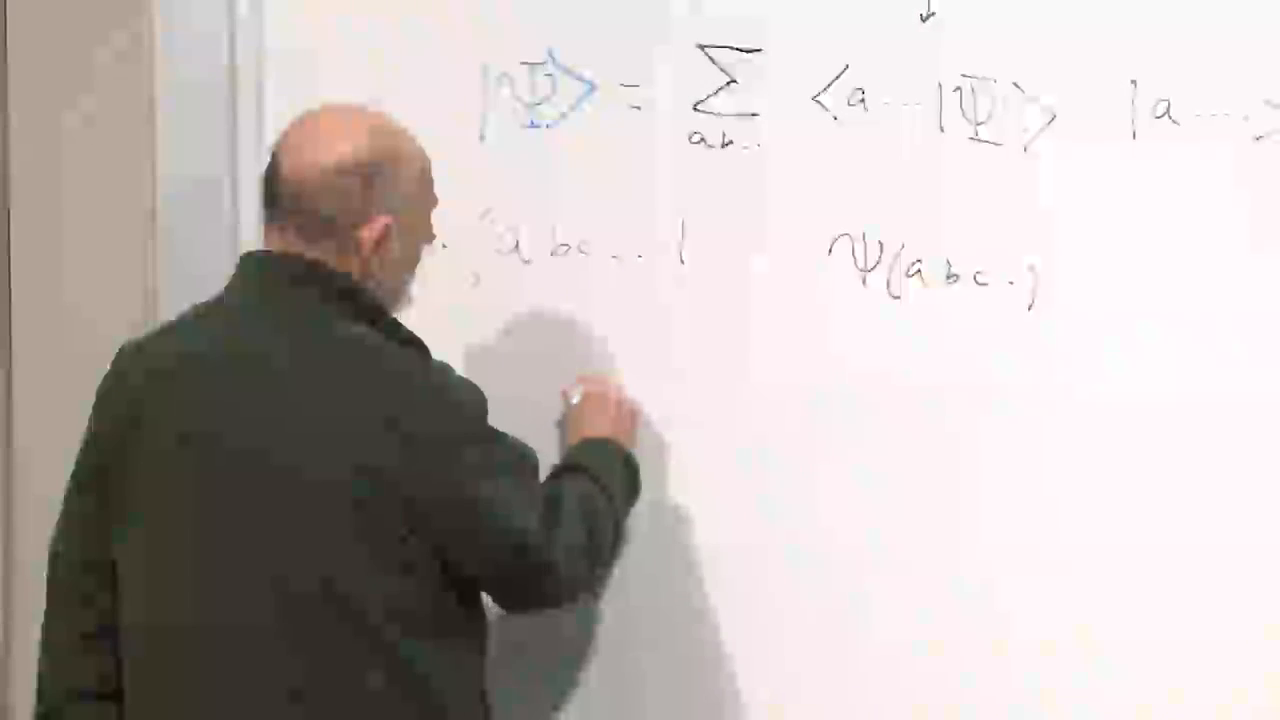
\includegraphics[width=0.88\textwidth]{lecture_07_figure_02.png}
\caption{Выражение для среднего значения, развернутое по коэффициентам волновой функции и матричным элементам.}
\lectureframe{00:14:08}
\end{figure}

Теперь разделим систему на часть Алисы и часть Боба. Пусть \(a\) — полная базисная метка для Алисы, а \(b\) — для Боба:
\begin{equation}
\ket{\Psi}_{AB}
=\sum_{a,b}\Psi(a,b)\ket{a,b}.
\label{eq:l7-composite-expansion}
\end{equation}
Наблюдаемая, относящаяся только к Алисе, представляется в составном пространстве как
\begin{equation}
L_A=L\otimes I_B,
\end{equation}
поэтому ее матричные элементы равны
\begin{equation}
\bra{a',b'}L_A\ket{a,b}
=L_{a'a}\delta_{b'b}.
\label{eq:l7-alice-local-matrix}
\end{equation}
Аналогично, локальная наблюдаемая Боба имеет вид
\begin{equation}
M_B=I_A\otimes M,
\qquad
\bra{a',b'}M_B\ket{a,b}
=\delta_{a'a}M_{b'b}.
\label{eq:l7-bob-local-matrix}
\end{equation}
Единичный оператор в нетронутом множителе — это математическая запись того, что операция Алисы действует на Алису, а операция Боба действует на Боба.

Подстановка уравнения~\eqref{eq:l7-alice-local-matrix} в выражение для среднего значения дает
\begin{equation}
\expect{L_A}
=\sum_{a',a,b}
\Psi^*(a',b)L_{a'a}\Psi(a,b).
\label{eq:l7-local-expectation}
\end{equation}
Эта формула уже содержит редуцированную матрицу плотности; мы перегруппируем ее после того, как сначала увидим, что происходит при факторизации.

\begin{classroomqa}
\audiencequestion{Почему в уравнении~\eqref{eq:l7-local-expectation} остается только один индекс Боба?}
\lecturerresponse{Единичный оператор в пространстве Боба дает \(\delta_{b'b}\). Он приравнивает метки bra и ket на стороне Боба, так что двойная сумма по \(b',b\) схлопывается в одну сумму по \(b\).}
\end{classroomqa}

\begin{classroomqa}
\audiencequestion{Нужно ли Алисе знать, какой базис использует Боб?}
\lecturerresponse{Ни одно физическое предсказание не зависит от базиса Боба. Сумма по полному базису Боба дает разложение единицы. Другой базис Боба меняет отдельные компоненты \(\Psi(a,b)\), но не среднее значение Алисы.}
\end{classroomqa}

\section{Состояния-произведения и корреляции}

В состоянии-произведении совместная волновая функция факторизуется:
\begin{equation}
\Psi(a,b)=\psi_A(a)\phi_B(b).
\label{eq:l7-wavefunction-factorization}
\end{equation}
Подставляя это в уравнение~\eqref{eq:l7-local-expectation}, получаем:
\begin{align}
\expect{L_A}
&=\sum_{a',a,b}
\psi_A^*(a')\phi_B^*(b)
L_{a'a}
\psi_A(a)\phi_B(b) \\
&=\left[
\sum_{a',a}\psi_A^*(a')L_{a'a}\psi_A(a)
\right]
\left[
\sum_b|\phi_B(b)|^2
\right] \\
&=\bra{\psi_A}L\ket{\psi_A}.
\label{eq:l7-product-local-expectation}
\end{align}
Нормировка Боба делает его множитель равным единице. Поэтому у Алисы в точности та же локальная статистика, которая была бы у нее, если бы система Боба вообще не была введена.

\begin{figure}[htbp]
\centering
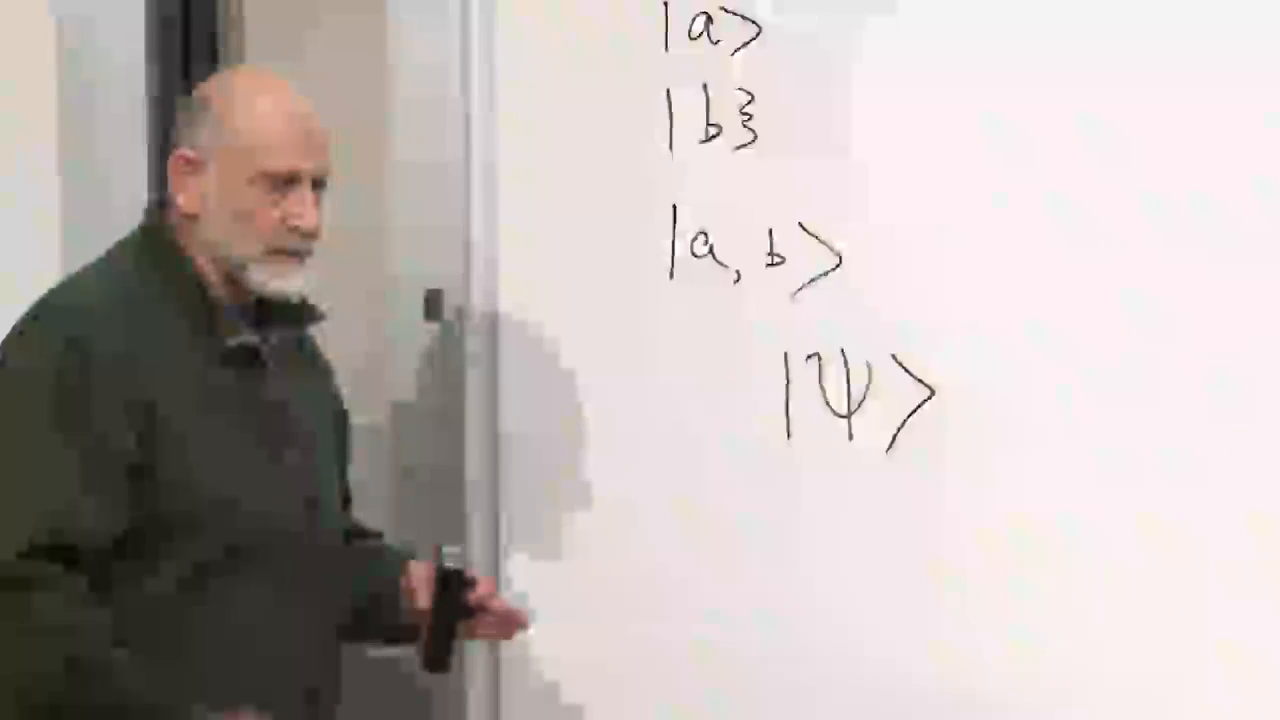
\includegraphics[width=0.88\textwidth]{lecture_07_figure_03.png}
\caption{Факторизация совместной волновой функции и соответствующее разделение локальных средних значений.}
\lectureframe{00:29:18}
\end{figure}

Произведение одной наблюдаемой Алисы и одной наблюдаемой Боба имеет матричные элементы
\begin{equation}
\bra{a',b'}L_A M_B\ket{a,b}
=L_{a'a}M_{b'b}.
\end{equation}
Для состояния-произведения его среднее значение факторизуется:
\begin{equation}
\expect{L_A M_B}
=\expect{L_A}\expect{M_B}.
\label{eq:l7-product-correlation-factorization}
\end{equation}
Поэтому естественно определить связную корреляцию
\begin{equation}
C(L,M)
=\expect{L_A M_B}
-\expect{L_A}\expect{M_B}.
\label{eq:l7-connected-correlation}
\end{equation}
Каждое состояние-произведение имеет \(C(L,M)=0\) для любой пары локальных наблюдаемых. Обратно, для чистого бипартитного состояния запутанность гарантирует, что для некоторой пары локальных наблюдаемых связная корреляция отлична от нуля.

\begin{classroomqa}
\audiencequestion{Означает ли \(L_A M_B\), что сначала измеряют Боба, а потом Алису?}
\lecturerresponse{Нет. Операторы действуют на векторы состояния; измерения выполняют приборы. Произведение означает, что сначала действует \(M_B\), а затем \(L_A\). Поскольку операторы занимают разные тензорные множители, \([L_A,M_B]=0\), так что их математический порядок несущественен. Лабораторный протокол оценки совместного среднего значения — отдельный вопрос.}
\end{classroomqa}

\begin{classroomqa}
\audiencequestion{Может ли состояние быть запутанным, даже когда одна выбранная корреляция обращается в нуль?}
\lecturerresponse{Безусловно. То, что один \(C(L,M)\) равен нулю, говорит лишь о том, что эта конкретная пара наблюдаемых некоррелирована. Чтобы установить факторизацию чистого состояния, должны факторизоваться все локальные перекрестные корреляции. Частичная корреляция также не обязана означать частичную запутанность в каком-либо простом одночисловом смысле; эту информацию несет полный спектр редуцированной матрицы плотности.}
\end{classroomqa}

\begin{classroomqa}
\audiencequestion{Всякое ли коррелированное состояние запутано?}
\lecturerresponse{Для обсуждаемых чистых состояний нефакторизующиеся корреляции выявляют запутанность. Для смешанных состояний обычные классические корреляции тоже могут делать \(C(L,M)\neq0\). Поэтому последующий критерий через матрицу плотности должен сопровождаться оговоркой о том, известно ли, что состояние целого является чистым.}
\end{classroomqa}

\section{Синглет: определенное целое с неопределенными частями}

Пусть \(\boldsymbol{\sigma}\) действует на спин Боба, а \(\boldsymbol{\tau}\) — на спин Алисы. Их синглетное состояние имеет вид
\begin{equation}
\ket{S}
=\frac{1}{\sqrt2}
\left(\ket{u d}-\ket{d u}\right),
\label{eq:l7-singlet}
\end{equation}
где первое место относится к Бобу, а второе — к Алисе. Ни один из спинов не имеет определенной \(z\)-компоненты:
\begin{equation}
\expect{\sigma_z}=0,
\qquad
\expect{\tau_z}=0.
\label{eq:l7-singlet-local-z}
\end{equation}
Однако их произведение определено:
\begin{equation}
\expect{\sigma_z\tau_z}=-1.
\label{eq:l7-singlet-product-z}
\end{equation}
При каждом измерении \(z\) получаются противоположные результаты.

Инвариантность относительно вращений делает это утверждение независимым от направления. Для любого единичного вектора \(\mathbf n\),
\begin{equation}
\expect{\boldsymbol{\sigma}\cdot\mathbf n}
=\expect{\boldsymbol{\tau}\cdot\mathbf n}=0,
\qquad
\expect{
(\boldsymbol{\sigma}\cdot\mathbf n)
(\boldsymbol{\tau}\cdot\mathbf n)
}=-1.
\label{eq:l7-singlet-any-axis}
\end{equation}
Более общо,
\begin{equation}
\expect{\sigma_i\tau_j}=-\delta_{ij}.
\label{eq:l7-singlet-correlation-tensor}
\end{equation}
Каждая подсистема полностью неполяризована, тогда как результаты при одинаковых осях идеально антикоррелированы.

\begin{figure}[htbp]
\centering
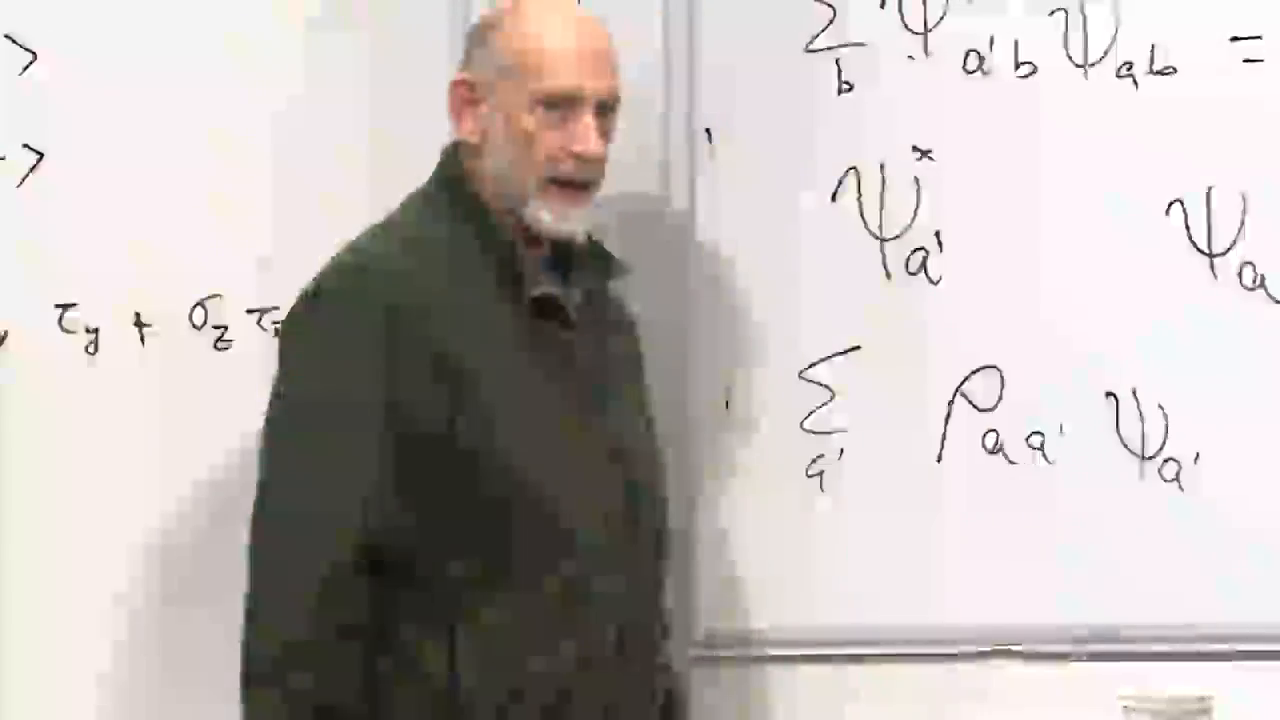
\includegraphics[width=0.88\textwidth]{lecture_07_figure_04.png}
\caption{Для синглета среднее значение каждого локального спина равно нулю, тогда как произведение одинаковых компонент равно \(-1\).}
\lectureframe{00:38:28}
\end{figure}

Это характерный переворот, порождаемый запутанностью. Для изолированного спина в чистом состоянии существует некоторое направление, вдоль которого его спин определён. В синглете ни одно направление не делает определённым ни один из локальных спинов. Тем не менее состояние составной системы является чистым и полностью заданным. Мы знаем о целом столько, сколько вообще допускает квантовая механика, и всё же не можем приписать чистое состояние ни одной из частей.

\begin{classroomqa}
\audiencequestion{Если состояние целого известно точно, почему мы не можем вывести определённое состояние для каждого спина?}
\lecturerresponse{Потому что синглет не является произведением. Его коэффициенты не раскладываются в амплитуду Боба, умноженную на амплитуду Алисы. Информация заключена в соотношениях между частями, а не в двух независимо существующих локальных волновых функциях.}
\end{classroomqa}

\begin{classroomqa}
\audiencequestion{Может ли оператор, такой как \(\sigma_z\), сам по себе быть возможным состоянием спина?}
\lecturerresponse{Нет. Состояние — это вектор или, более общо, оператор плотности; \(\sigma_z\) — наблюдаемая, действующая на состояния. Собственный вектор \(\sigma_z\) — это состояние с определённой \(z\)-компонентой спина, но наблюдаемая и её собственные векторы — объекты разных типов.}
\end{classroomqa}

\begin{classroomqa}
\audiencequestion{Когда мы записываем \(\sigma_z\tau_z\ket{S}=-\ket{S}\), выполнили ли мы измерение?}
\lecturerresponse{Нет. Это уравнение фиксирует, как оператор действует на вектор. Оно говорит нам, что измерение соответствующей совместной наблюдаемой наверняка дало бы \(-1\), но простая запись уравнения на собственные значения ещё не включает никакого детектора.}
\end{classroomqa}

\begin{classroomqa}
\audiencequestion{Может ли запутанная пара быть лишь частично коррелированной?}
\lecturerresponse{Да. Идеальная антикорреляция — особое свойство синглета для одинаковых осей. Другие запутанные состояния могут иметь более слабые корреляции, и даже синглет даёт \(-\mathbf a\cdot\mathbf b\), а не \(-1\), когда две оси различны. Запутанность связана с нефакторизуемостью, а не с полным совпадением или несовпадением в каждом выбранном измерении.}
\end{classroomqa}

\section{Подготовка синглета посредством энергетической релаксации}

Инвариантный относительно вращений двухспиновый оператор
\begin{equation}
\boldsymbol{\sigma}\cdot\boldsymbol{\tau}
=\sigma_x\tau_x+\sigma_y\tau_y+\sigma_z\tau_z
\label{eq:l7-spin-dot-spin}
\end{equation}
структурирует четырёхмерное пространство состояний. Для синглета
\begin{equation}
(\boldsymbol{\sigma}\cdot\boldsymbol{\tau})\ket{S}
=-3\ket{S},
\label{eq:l7-singlet-dot-eigenvalue}
\end{equation}
тогда как каждое из трёх триплетных состояний имеет собственное значение \(+1\).

\begin{figure}[htbp]
\centering
\includegraphics[width=0.88\textwidth]{lecture_07_figure_05.png}
\caption{Инвариантное относительно вращений взаимодействие \(\boldsymbol{\sigma}\cdot\boldsymbol{\tau}\) и его роль в разделении синглетного и триплетного секторов.}
\lectureframe{00:52:33}
\end{figure}

Предположим, что гамильтониан взаимодействия содержит
\begin{equation}
H_{\mathrm{int}}
=J\,\boldsymbol{\sigma}\cdot\boldsymbol{\tau}.
\label{eq:l7-exchange-hamiltonian}
\end{equation}
Для антиферромагнитной связи \(J>0\) синглет лежит ниже триплета на
\begin{equation}
\Delta E=4J.
\end{equation}
Сблизьте спины, дайте компонентам с более высокой энергией релаксировать с испусканием фотона, фонона или какого-либо другого возбуждения, и пара релаксирует к синглету. Затем спины можно разнести, сохранив их совместное состояние, при условии что разделение не вносит неконтролируемых вращений спина и не закрывает энергетическую щель слишком резко.

Та же энергетическая логика проявляется и в атомных системах. Например, в позитронии спиновая связь электрона и позитрона расщепляет синглетную и триплетную конфигурации. Разность энергий одновременно является и разностью масс согласно \(E=mc^2\), хотя в спектроскопии это расщепление обычно выражают как энергию или частоту.

\begin{classroomqa}
\audiencequestion{Всегда ли синглет является основным состоянием двух взаимодействующих спинов?}
\lecturerresponse{Нет. Он является основным состоянием при знаке \(J>0\) в уравнении~\eqref{eq:l7-exchange-hamiltonian}. Если поменять знак, ниже по энергии окажется триплет. Аргумент о подготовке зависит от конкретного взаимодействия и порядка его энергий, а не просто от самого существования двух спинов.}
\end{classroomqa}

\begin{classroomqa}
\audiencequestion{Можно ли измерить \(\boldsymbol{\sigma}\cdot\boldsymbol{\tau}\), отдельно измерив все три компоненты?}
\lecturerresponse{Не на одной паре посредством трёх одновременных локальных измерений спина: \(\sigma_x,\sigma_y,\sigma_z\) несовместимы, и три компоненты \(\tau\) тоже несовместимы. Его среднее значение можно восстановить по трём подансамблям, измеренным вдоль \(x,y,z\), либо синглет--триплетную наблюдаемую можно измерить непосредственно подходящим совместным прибором.}
\end{classroomqa}

\begin{classroomqa}
\audiencequestion{После разделения спинов должны ли они продолжать взаимодействовать, чтобы оставаться запутанными?}
\lecturerresponse{Нет. Взаимодействие нужно, чтобы подготовить или изменить состояние, но после того как синглет подготовлен, унитарная эволюция может сохранять его запутанность без непрерывно действующей силы между частицами. Локальные магнитные поля могут поворачивать оба фактора, однако локальные унитарные повороты сами по себе не уничтожают запутанность.}
\end{classroomqa}

\section{Редуцированная матрица плотности}

Вернёмся к локальному среднему значению Алисы:
\begin{equation}
\expect{L_A}
=\sum_{a',a,b}
\Psi^*(a',b)L_{a'a}\Psi(a,b).
\end{equation}
Перегруппируем множители, не относящиеся к \(L\):
\begin{equation}
\expect{L_A}
=\sum_{a',a}
\left[
\sum_b\Psi(a,b)\Psi^*(a',b)
\right]L_{a'a}.
\label{eq:l7-regrouped-expectation}
\end{equation}
Выражение в скобках есть редуцированная матрица плотности Алисы,
\begin{equation}
(\rho_A)_{aa'}
=\sum_b\Psi(a,b)\Psi^*(a',b).
\label{eq:l7-reduced-density-components}
\end{equation}
В базисно-независимой записи,
\begin{equation}
\rho_A
=\operatorname{Tr}_B\ket{\Psi}\bra{\Psi},
\label{eq:l7-partial-trace}
\end{equation}
и любое локальное для Алисы среднее значение равно
\begin{equation}
\expect{L_A}
=\operatorname{Tr}_A(\rho_A L).
\label{eq:l7-density-expectation}
\end{equation}

\begin{figure}[htbp]
\centering
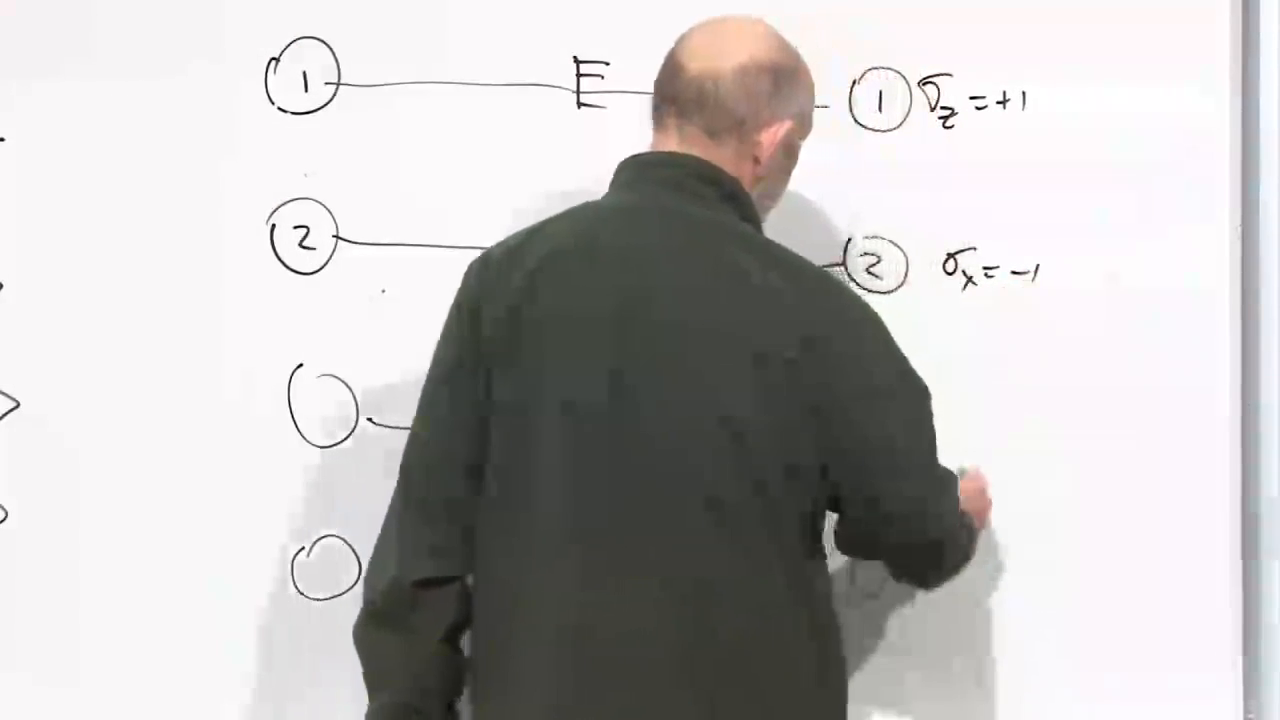
\includegraphics[width=0.88\textwidth]{lecture_07_figure_06.png}
\caption{Матрица плотности Алисы, получаемая суммированием совместных амплитуд по базисному индексу Боба.}
\lectureframe{01:02:33}
\end{figure}

Редуцированная матрица плотности эрмитова, положительна и нормирована:
\begin{equation}
\rho_A^\dagger=\rho_A,
\qquad
\bra{\chi}\rho_A\ket{\chi}\geq0,
\qquad
\operatorname{Tr}\rho_A=1.
\label{eq:l7-density-properties}
\end{equation}
Она содержит ровно ту информацию, которая нужна для всех измерений, ограниченных подсистемой Алисы. Если два глобальных состояния дают одну и ту же \(\rho_A\), никакой эксперимент только на стороне Алисы не сможет их различить.

\begin{classroomqa}
\audiencequestion{Измеряет ли Алиса матрицу плотности как одну наблюдаемую?}
\lecturerresponse{Не за один запуск. Матрица плотности — это объект, из которого вычисляются все вероятности локальных измерений. Имея много одинаково подготовленных систем, Алиса может восстановить её методом томографии: она измеряет достаточный набор наблюдаемых и выводит матрицу из их средних значений.}
\end{classroomqa}

\begin{classroomqa}
\audiencequestion{Почему суммируют по Бобу, а не выбирают одно из состояний Боба?}
\lecturerresponse{Потому что у Алисы нет информации о результате Боба. Частичный след суммирует по полному базису Боба и даёт необусловленное локальное состояние. Если вместо этого выбрать один результат Боба, получится условное состояние; это другая операция, и она требует знания этого результата.}
\end{classroomqa}

Для состояния-произведения \(\Psi(a,b)=\psi_A(a)\phi_B(b)\),
\begin{align}
(\rho_A)_{aa'}
&=\sum_b
\psi_A(a)\phi_B(b)
\psi_A^*(a')\phi_B^*(b) \\
&=\psi_A(a)\psi_A^*(a')
\sum_b|\phi_B(b)|^2 \\
&=\psi_A(a)\psi_A^*(a').
\end{align}
Следовательно,
\begin{equation}
\rho_A=\ket{\psi_A}\bra{\psi_A}.
\label{eq:l7-pure-projector}
\end{equation}
Это проектор ранга один. Действуя на \(\ket{\psi_A}\), получаем
\begin{equation}
\rho_A\ket{\psi_A}
=\ket{\psi_A}\braket{\psi_A}{\psi_A}
=\ket{\psi_A},
\label{eq:l7-density-on-state}
\end{equation}
тогда как для любого \(\ket{\chi}\), ортогонального \(\ket{\psi_A}\),
\begin{equation}
\rho_A\ket{\chi}
=\ket{\psi_A}\braket{\psi_A}{\chi}
=0.
\label{eq:l7-density-on-orthogonal}
\end{equation}

\begin{figure}[htbp]
\centering
\includegraphics[width=0.88\textwidth]{lecture_07_figure_07.png}
\caption{Матрица плотности состояния-произведения, действующая как проектор: собственное значение \(1\) вдоль \(\ket{\psi_A}\) и \(0\) на ортогональных векторах.}
\lectureframe{01:09:43}
\end{figure}

\section{Спектр матрицы плотности и запутанность}

Собственные значения \(\rho_A\) неотрицательны и в сумме дают единицу. Для чистого состояния целого:
\begin{itemize}
\item ровно одно ненулевое собственное значение, равное \(1\), означает, что состояние является состоянием-произведением;
\item более одного ненулевого собственного значения означает, что состояние запутано;
\item равные собственные значения на всём доступном локальном носителе соответствуют максимальной запутанности.
\end{itemize}
Это утверждение наиболее прозрачно видно из разложения Шмидта,
\begin{equation}
\begin{aligned}
\ket{\Psi}_{AB}
&=\sum_{r=1}^{R}\sqrt{\lambda_r}
\ket{r}_A\ket{r}_B,\\
\lambda_r&\geq0,
\qquad
\sum_r\lambda_r=1.
\end{aligned}
\label{eq:l7-schmidt}
\end{equation}
для которого
\begin{equation}
\rho_A=\sum_{r=1}^{R}\lambda_r\ket{r}_A\bra{r}.
\label{eq:l7-schmidt-density}
\end{equation}
Ранг Шмидта \(R\) равен единице для состояния-произведения и больше единицы для запутанного чистого состояния.

Для синглета,
\begin{equation}
\rho_A
=\operatorname{Tr}_B\ket{S}\bra{S}
=\frac12\ket{u}\bra{u}
+\frac12\ket{d}\bra{d}
=\frac12 I.
\label{eq:l7-singlet-reduced-density}
\end{equation}
Его собственные значения равны
\begin{equation}
\operatorname{spec}(\rho_A)
=\left\{\frac12,\frac12\right\}.
\end{equation}
Локальное состояние Алисы максимально смешано, хотя состояние пары является чистым.

Спектр подсказывает количественную меру. Энтропия фон Неймана
\begin{equation}
S(\rho_A)
=-\operatorname{Tr}(\rho_A\log\rho_A)
=-\sum_r\lambda_r\log\lambda_r
\label{eq:l7-entanglement-entropy}
\end{equation}
обращается в нуль для чистого состояния-произведения и достигает \(\log d_A\) для максимально запутанного состояния при \(d_A\leq d_B\). Подробное использование энтропии можно отложить; спектр уже даёт существенное различие.

\begin{classroomqa}
\audiencequestion{Должно ли каждое собственное значение запутанной редуцированной матрицы плотности быть ненулевым?}
\lecturerresponse{Нет. Достаточно более чем одного ненулевого собственного значения. Если пространство Алисы велико, запутанное состояние может занимать лишь подпространство Шмидта меньшей размерности, оставляя дополнительные нулевые собственные значения. Максимальная запутанность означает равенство собственных значений во всём пространстве меньшей подсистемы, а не просто равенство внутри произвольно выбранного поднабора.}
\end{classroomqa}

\begin{classroomqa}
\audiencequestion{Доказывает ли смешанная редуцированная матрица плотности сама по себе, что Алиса запутана с Бобом?}
\lecturerresponse{Только если известно, что глобальное состояние является чистым. Смешанное локальное состояние может также возникать из обычной классической смеси в смешанном глобальном состоянии. Однако для чистого бипартитного состояния локальная смешанность в точности эквивалентна запутанности относительно данного разбиения на две подсистемы.}
\end{classroomqa}

\begin{classroomqa}
\audiencequestion{Могут ли все моменты наблюдаемых Алисы определить её распределения вероятностей?}
\lecturerresponse{В конечномерной системе средние значения базиса операторов определяют \(\rho_A\), а \(\rho_A\) через правило Борна определяет каждое локальное распределение исходов. Для восстановления требуется ансамбль одинаково приготовленных копий; по одному изолированному событию матрицу плотности определить нельзя.}
\end{classroomqa}

\section{Измерение как запутывающее взаимодействие}

Заменим Алису и Боба спином и измерительным прибором. Пусть у прибора есть состояние готовности \(\ket{0}_D\) и сработавшее состояние \(\ket{1}_D\). Идеальное взаимодействие, регистрирующее, направлен ли спин вверх, можно представить так:
\begin{align}
\ket{u}\ket{0}_D&\longrightarrow\ket{u}\ket{1}_D,\\
\ket{d}\ket{0}_D&\longrightarrow\ket{d}\ket{0}_D.
\label{eq:l7-measurement-basis-map}
\end{align}
Детектор должен начинать в известном состоянии готовности; иначе его конечное состояние не давало бы однозначной записи.

Линейность фиксирует эволюцию суперпозиции:
\begin{equation}
\left(\alpha\ket{u}+\beta\ket{d}\right)\ket{0}_D
\longrightarrow
\alpha\ket{u}\ket{1}_D
+\beta\ket{d}\ket{0}_D.
\label{eq:l7-measurement-entanglement}
\end{equation}
Если ни один из коэффициентов не обращается в нуль, конечное состояние запутано. Прибор получил информацию именно потому, что состояние его указателя коррелировано со спином.

\begin{figure}[htbp]
\centering
\includegraphics[width=0.88\textwidth]{lecture_07_figure_08.png}
\caption{Идеальное измерение сопоставляет альтернативам спина различные состояния указателя и тем самым создаёт запутанность.}
\lectureframe{01:20:20}
\end{figure}

Если оставить только спин и не учитывать детектор, его редуцированное состояние имеет вид
\begin{equation}
\rho_{\mathrm{spin}}
=|\alpha|^2\ket{u}\bra{u}
+|\beta|^2\ket{d}\bra{d},
\label{eq:l7-postmeasurement-reduced-state}
\end{equation}
если считать записи указателя ортогональными. Интерференционные члены исчезли из локального описания, потому что они хранятся в корреляциях с прибором.

Теперь есть два взаимодополнительных описания. Если результат детектора считывается и проводится обусловливание по записи, спину приписывается соответствующая ветвь: \(\ket{u}\) после срабатывания или \(\ket{d}\) после отсутствия срабатывания. Это описание с коллапсом. Если детектор и спин рассматриваются как одна замкнутая система, то ~\eqref{eq:l7-measurement-entanglement} — это обычная унитарная эволюция, и ни одна ветвь не была удалена из совместного состояния.

\begin{classroomqa}
\audiencequestion{Есть ли в измерении нечто большее, чем запутанность?}
\lecturerresponse{На уровне динамики системы--прибора измерение — это взаимодействие, устанавливающее надёжную корреляцию. Коллапс — это условное описание, используемое после того, как выбрана определённая запись. Считать ли такое обновление фундаментальным или относительным к выбранной границе раздела — вопрос интерпретации; операциональные предсказания совпадают.}
\end{classroomqa}

\begin{classroomqa}
\audiencequestion{Почему идеальное измерение оставляет собственное состояние спина неизменным?}
\lecturerresponse{Это требование повторяемости для данной модели. Если вход уже является собственным состоянием измеряемой наблюдаемой, прибор должен зарегистрировать её значение, не изменяя его. Реальные измерения могут быть разрушающими, но тогда их взаимодействие нужно моделировать иначе.}
\end{classroomqa}

\section{Иерархия наблюдателей}

Если признать прибор квантовой системой, нет естественной причины останавливаться на этом. Свет от указателя взаимодействует с глазом; сигналы от глаза коррелируются с мозгом; за одним наблюдателем может наблюдать другой. Кот Schr\"odinger и друг Вигнера наглядно иллюстрируют ту же вложенную структуру:
\begin{equation}
\begin{gathered}
\text{spin}
\longrightarrow
\text{apparatus}
\longrightarrow
\text{cat}\\
\longrightarrow
\text{Schr\"odinger}
\longrightarrow
\text{Wigner}.
\end{gathered}
\label{eq:l7-observer-chain}
\end{equation}
Внутри любой выбранной границы эту цепочку можно описывать унитарной эволюцией и растущей запутанностью. Вне неё используют язык коллапса, обусловленного результатом.

Ключевое условие согласованности состоит в том, что границу можно перемещать. Если кот регистрирует спин вверх, то Schr\"odinger должен позднее зарегистрировать кота, увидевшего спин вверх, а Вигнер должен зарегистрировать Schr\"odinger, регистрирующего ту же историю. Квантовая механика не выделяет единственную чёткую границу, на которой нужно считать, что произошло объективное событие. Коты, глаза и мозги состоят из физических степеней свободы; исключение одного из них из квантовой механики потребовало бы дополнительного закона.

Отношение Фейнмана к возникающему из-за этого дискомфорту было прагматическим. Концептуальная проблема может быть настолько велика, что трудно даже сформулировать, существует ли она вообще, тогда как вычислительные правила продолжают предсказывать каждый эксперимент, к которому они применимы. Назначение формализма не в том, чтобы навязать одну интерпретацию, а в том, чтобы точно указать источник дискомфорта: полное знание о целом может сосуществовать с отсутствием у его частей какого-либо описания чистым состоянием.

\begin{classroomqa}
\audiencequestion{Если я — кот, должен ли я проводить границу по самому себе?}
\lecturerresponse{Вы можете использовать описание с коллапсом для той определённой записи, которая вам доступна. Другой наблюдатель, включающий вас в более крупную изолированную систему, может использовать описание в терминах запутанного состояния. Требуется не чтобы все проводили одну и ту же границу, а чтобы все описания давали согласованные записи всякий раз, когда наблюдатели позднее сравнивают результаты.}
\end{classroomqa}

\begin{classroomqa}
\audiencequestion{Где происходит объективное событие: у атома, у кота, у Schr\"odinger или у Вигнера?}
\lecturerresponse{Унитарный формализм не выделяет ни одно из этих мест как привилегированную границу. Возможно, обычные слова вроде \emph{происходит} используются уже вне того контекста, в котором они точны. Формальные средства говорят нам, как распространяются корреляции и что может предсказать каждый наблюдатель; решать, как интерпретировать последнюю границу, — отдельная задача.}
\end{classroomqa}

\subsection{Слабое взаимодействие и несовершенное считывание}

Идеальное отображение в ~\eqref{eq:l7-measurement-basis-map} создаёт полностью различимые записи. Более слабое взаимодействие может оставлять состояния прибора лишь частично различимыми:
\begin{equation}
\alpha\ket{u}\ket{D_u}
+\beta\ket{d}\ket{D_d},
\qquad
0<|\braket{D_d}{D_u}|<1.
\label{eq:l7-weak-measurement}
\end{equation}
Тогда прибор получает лишь частичную информацию, а запутанность неполна. Это ситуация слабого или нечёткого измерения.

Эту ситуацию нужно отличать от плохого считывания на последующих этапах. Детектор мог полностью скоррелироваться со спином, тогда как глаз, кабель, усилитель или мозг не смогли без искажений передать запись. В первом случае взаимодействие системы--детектора слабо; во втором у детектора существует хорошая запись, но последующая передача информации неэффективна. Эффективность детектора может зависеть от любой из этих стадий, поэтому, прежде чем приписывать причину, нужно определить соответствующее физическое взаимодействие.

\begin{classroomqa}
\audiencequestion{Если из-за плохого зрения показание указателя неопределённо, было ли квантовое измерение слабым?}
\lecturerresponse{Не обязательно. Спин мог быть сильно и полностью скоррелирован с прибором, тогда как канал от прибора к глазу или от глаза к мозгу был плохим. По-настоящему слабое измерение означает, что начальное взаимодействие системы--прибора само породило лишь частично различимые записи.}
\end{classroomqa}

\section{Локальность и отсутствие сигнализации}

Выражению \emph{действие на расстоянии} следует придать операциональный смысл. В обычной физике далёкое воздействие меняет то, что можно наблюдать здесь. Если бы Солнце исчезло и движение Земли изменилось немедленно, а не после времени распространения света, это изменение можно было бы использовать для передачи информации быстрее света. Это была бы подлинная нелокальная сигнализация.

Запутанность не допускает такой сигнализации. Пусть Боб выполняет локальную квантовую операцию, представленную операторами Крауса \(K_\mu\), причём
\begin{equation}
\sum_\mu K_\mu^\dagger K_\mu=I_B.
\end{equation}
Если Алиса не узнаёт исход Боба, конечное совместное состояние равно
\begin{equation}
\rho'_{AB}
=\sum_\mu
(I_A\otimes K_\mu)\rho_{AB}
(I_A\otimes K_\mu^\dagger).
\end{equation}
Взятие частичного следа по Бобу даёт
\begin{equation}
\rho'_A
=\operatorname{Tr}_B\rho'_{AB}
=\operatorname{Tr}_B\rho_{AB}
=\rho_A.
\label{eq:l7-no-signaling}
\end{equation}
Следовательно, никакая безусловная локальная вероятность Алисы не меняется от выбора Бобом локальной операции, сохраняющей след.

С условными состояниями дело обстоит иначе. Если Боб измеряет и получает исход \(\mu\), Алиса может приписать
\begin{equation}
\rho_{A|\mu}
=\frac{
\operatorname{Tr}_B\!\left[
(I_A\otimes K_\mu)\rho_{AB}
(I_A\otimes K_\mu^\dagger)
\right]
}{p_\mu}.
\label{eq:l7-conditioned-state}
\end{equation}
Но Алиса не может знать, какое именно \(\rho_{A|\mu}\) применимо, пока Боб не сообщит \(\mu\) обычным сигналом. До прихода сообщения она должна усреднить по исходам:
\begin{equation}
\sum_\mu p_\mu\rho_{A|\mu}=\rho_A.
\label{eq:l7-conditioned-average}
\end{equation}

\begin{classroomqa}
\audiencequestion{Когда меняется матрица плотности Алисы, если Боб измеряет первым?}
\lecturerresponse{Её безусловная матрица плотности не меняется. Когда до неё доходит результат Боба, она может заменить её соответствующей условной матрицей плотности. Это обновление отражает ставшую доступной новую информацию и не может использоваться до прибытия классического сообщения.}
\end{classroomqa}

\begin{classroomqa}
\audiencequestion{Приводит ли измерение Боба к физическому коллапсу состояния Алисы в тот же момент?}
\lecturerresponse{Разные интерпретации по-разному описывают это условное обновление, но все согласны в проверяемом утверждении: локальные вероятности исходов Алисы остаются неизменными, пока ей не становится доступной информация от Боба. Никакого управляемого мгновенного сигнала не возникает.}
\end{classroomqa}

Представьте себе множество синглетных пар, расположенных по пронумерованным строкам. В одном ряду Боб измеряет \(z\), в другом \(x\), в третьем \(y\) и так далее. Локальные результаты Алисы остаются несмещённой последовательностью в каждой строке:
\begin{equation}
P_A(+|\mathbf a)=P_A(-|\mathbf a)=\frac12.
\label{eq:l7-alice-marginal}
\end{equation}
Ничто в её тетради не показывает, какие оси выбрал Боб и какие исходы он получил.

\begin{figure}[htbp]
\centering
\includegraphics[width=0.88\textwidth]{lecture_07_figure_09.png}
\caption{Многие независимо подготовленные пары позволяют назначать разным строкам разные оси измерения; маргинальная статистика Алисы при этом не меняется.}
\lectureframe{01:49:00}
\end{figure}

После того как приходит телеграмма, идущая не быстрее света, с указанием для каждой строки оси Боба и его результата, Алиса может отсортировать свои записи. Тогда измерения синглета по одинаковым осям окажутся попарно противоположными. Сообщение выявляет корреляции, уже присутствующие в совместной статистике; оно не изменяет задним числом более раннее локальное распределение частот Алисы.

\begin{classroomqa}
\audiencequestion{Может ли Алиса по достаточно большому числу моментов своих собственных данных определить выбор Боба?}
\lecturerresponse{Нет. Все локальные для Алисы моменты фиксируются \(\rho_A\), а уравнение~\eqref{eq:l7-no-signaling} оставляет эту матрицу неизменной. Большее число копий улучшает её оценку той же локальной матрицы плотности; базис или результат Боба они не раскрывают.}
\end{classroomqa}

\begin{classroomqa}
\audiencequestion{Что если Боб выбирает разную ось для каждого элемента ансамбля?}
\lecturerresponse{Алиса всё равно видит то же локальное распределение. Когда Боб пришлёт настройки и результаты построчно, обе стороны смогут сравнить условные корреляции для каждой пары осей. Зависимость от настройки проявляется в совместной статистике, а не в маргинальной статистике Алисы.}
\end{classroomqa}

\section{Вопрос Белла как задача моделирования}

Различие между отсутствием сигнализации и белловской нелокальностью становится яснее, если рассматривать его как задачу классического моделирования. Начнём с одного спина:
\begin{equation}
\ket{\psi}=\alpha_u\ket{u}+\alpha_d\ket{d},
\qquad
|\alpha_u|^2+|\alpha_d|^2=1.
\end{equation}
Классическая программа может хранить две комплексные амплитуды, эволюционировать их по уравнению Schr\"odinger и принимать выбранное пользователем направление измерения. Когда подаётся команда измерения, программа вычисляет вероятности Борна, использует генератор псевдослучайных чисел для выбора результата, выводит этот результат и обновляет хранимое состояние до соответствующего собственного состояния. Повторение процесса воспроизводит статистику одного спина.

Следовательно, сама по себе случайность не является границей между классической и квантовой механикой. Классические компьютеры могут генерировать последовательности, которые в операциональном смысле достаточно случайны для моделирования, даже если лежащие в их основе псевдослучайные алгоритмы детерминированы.

Для двух спинов в состоянии-произведении также достаточно двух разнесённых компьютеров. Компьютер Алисы хранит и эволюционирует \(\ket{\psi_A}\); компьютер Боба — \(\ket{\phi_B}\). Каждый реагирует только на свою локальную настройку. Поскольку совместные вероятности факторизуются, после разделения компьютеров никакая связь не нужна.

Запутанная пара меняет задачу. Можно свести обе машины вместе перед экспериментом, загрузить в них коррелированные скрытые данные, синхронизировать их часы и даже задать им одинаковые начальные значения генератора случайных чисел. После разделения, однако, каждый выход должен зависеть только от своей локальной настройки измерения и общей информации, сообщённой заранее. Теорема Белла показывает, что никакая такая локальная схема со скрытыми переменными не воспроизводит все квантовые корреляции при свободно выбираемых настройках.

\begin{figure}[htbp]
\centering
\includegraphics[width=0.88\textwidth]{lecture_07_figure_10.png}
\caption{Модель с разнесёнными компьютерами: локальные программы могут иметь общие данные о подготовке, но после разделения они не могут обмениваться настройками измерения.}
\lectureframe{02:00:00}
\end{figure}

Если между компьютерами остаются провода, так что настройками и результатами можно обмениваться, моделирование может воспроизвести корреляции. Но тогда эта пара уже не является по-настоящему разделённой локальной моделью; она функционирует как один связанный компьютер. Препятствие заключается не в классических вычислениях как таковых. Одна глобальная классическая машина может моделировать конечные квантовые системы, храня полную совместную волновую функцию, хотя требуемая память обычно растёт экспоненциально с числом подсистем. Препятствие Белла касается разложения на локальные машины, работающие независимо.

\begin{classroomqa}
\audiencequestion{Почему двум компьютерам нельзя просто использовать одну и ту же последовательность случайных чисел?}
\lecturerresponse{Общая случайность уже допускается в локальной модели со скрытыми переменными. Она может заранее предопределять коррелированные ответы, но каждый ответ должен подходить для любой настройки измерения, которая позднее может быть выбрана на данной стороне. Неравенства Белла выражают ограничения, которым подчиняются все такие заранее согласованные локальные стратегии; квантовые корреляции нарушают эти ограничения.}
\end{classroomqa}

\begin{classroomqa}
\audiencequestion{Должны ли случайные числа зависеть от направлений измерения?}
\lecturerresponse{Локальный результат может зависеть от собственного локального направления и общих скрытых данных, но не от удалённого направления, выбранного после разделения. Допущение зависимости от обеих настроек требует связи, ретрокаузальности или нарушения обычного предположения о независимости выбора измерения. Теорема Белла делает эти предположения явными, вместо того чтобы прятать их за словом \emph{случайный}.}
\end{classroomqa}

\begin{classroomqa}
\audiencequestion{Могли бы два разнесённых квантовых компьютера преуспеть там, где классические программы терпят неудачу?}
\lecturerresponse{Они могут преуспеть, если имеют общие запутанные квантовые степени свободы. В этом случае компьютеры не моделируют запутанность при помощи локальных классических записей; они физически ею обладают. Их локальные результаты по-прежнему не могут передать управляемое сверхсветовое сообщение.}
\end{classroomqa}

\begin{classroomqa}
\audiencequestion{Может ли один обычный классический компьютер смоделировать всю пару целиком?}
\lecturerresponse{Да. Он может хранить четыре совместные амплитуды и вычислять все вероятности измерений в одном месте. Для многих частиц такое прямое моделирование становится затратным, потому что размерность гильбертова пространства растёт экспоненциально, но никакого противоречия с Беллом не возникает, когда вся информация глобально доступна внутри одной машины.}
\end{classroomqa}

\begin{classroomqa}
\audiencequestion{Следовательно, доказывает ли теорема Белла обычное действие на расстоянии?}
\lecturerresponse{Она доказывает, что локальные объяснения со скрытыми переменными, удовлетворяющие предпосылкам Белла, не могут воспроизвести наблюдаемые корреляции. Она не предоставляет Алисе или Бобу канала сверхсветовой сигнализации. Белловская нелокальность и операциональная передача сигналов быстрее света — различные утверждения.}
\end{classroomqa}

\section{Что можно узнать локально?}

Нельзя смешивать локальные и совместные наблюдаемые. Боб может измерить \(\sigma_x\), а Алиса — \(\tau_x\); позже, сравнив записи, они оценивают
\begin{equation}
\expect{\sigma_x\tau_x}.
\end{equation}
Ни один из локальных приборов по отдельности не измеряет это произведение. Скаляр относительно вращений
\begin{equation}
\boldsymbol{\sigma}\cdot\boldsymbol{\tau}
=\sigma_x\tau_x+\sigma_y\tau_y+\sigma_z\tau_z
\end{equation}
требует либо разных подансамблей для трёх слагаемых, либо нового совместного прибора, различающего синглетный и триплетный секторы. Нельзя получить все три несовместимых произведения компонент из одной пары с помощью исходных локальных спиновых измерителей.

\begin{classroomqa}
\audiencequestion{Существуют ли наблюдаемые всей системы, которые исходные приборы Алисы и Боба не могут измерить по отдельности?}
\lecturerresponse{Да. Отдельное произведение, такое как \(\sigma_x\tau_x\), можно оценить по двум локальным \(x\)-измерениям с последующим сравнением. Сумму \(\boldsymbol{\sigma}\cdot\boldsymbol{\tau}\) нельзя составить из одновременных показаний \(x,y,z\) на одной паре. Для неё требуется подлинно совместное синглетное--триплетное измерение или отдельные ансамбли для несовместимых слагаемых.}
\end{classroomqa}

Боб не может сделать вывод о запутанности по одному событию. Однако по многим одинаково подготовленным копиям он может восстановить свою редуцированную матрицу плотности. Для кубита,
\begin{equation}
\rho_B
=\frac12\left(
I+\mathbf r\cdot\boldsymbol{\sigma}
\right),
\label{eq:l7-bloch-density}
\end{equation}
измерения вдоль нескольких осей определяют вектор Блоха \(\mathbf r\). Если \(|\mathbf r|=1\), локальное состояние Боба чистое; если \(|\mathbf r|<1\), оно смешанное. В частном случае, когда известно, что глобальная подготовка в каждом испытании даёт одно и то же чистое состояние, локальная смешанность доказывает, что Боб запутан с чем-то вне его подсистемы.

Для состояния-произведения двух чистых спинов Боб может искать направление поляризации \(\mathbf n=\mathbf r/|\mathbf r|\). Вдоль этой оси повторные измерения дают один определённый ответ. Для синглета \(\mathbf r=0\), поэтому любая ось остаётся локально случайной. Такой поиск никогда не находит направления поляризации.

\begin{classroomqa}
\audiencequestion{Может ли Боб обнаружить запутанность, не разговаривая с Алисой?}
\lecturerresponse{По ансамблю он может обнаружить, что его собственное редуцированное состояние смешано. Если он также знает, что каждая пара была подготовлена в одном и том же глобальном чистом состоянии, он может заключить о наличии запутанности между подсистемами. Без этого предположения о чистоте его смешанное состояние могло бы вместо этого происходить из классической смеси подготовок, и одни лишь локальные данные не позволили бы провести это различие.}
\end{classroomqa}

\begin{classroomqa}
\audiencequestion{Почему необходимы многие одинаково подготовленные системы?}
\lecturerresponse{Каждое измерение спина даёт только один исход и, как правило, возмущает эту копию. Поэтому томография распределяет несовместимые измерения по ансамблю, подготовленному одной и той же процедурой. Матрица плотности и её спектр — это статистические свойства, выводимые из этих повторных испытаний, а не метки, раскрываемые одной частицей.}
\end{classroomqa}

Логика теперь замыкается там, где началась. Запутанность — это не некое расплывчатое совместное обладание состоянием. Это то, что чистое совместное состояние не факторизуется; локально это проявляется как редуцированная матрица плотности, не являющаяся проектором, а совместно — как корреляции, которые нельзя воспроизвести раздельным классическим учётом. Целое может быть в точности известно, тогда как каждая часть остаётся смешанной. Этот факт делает измерение возможным, сохраняет отсутствие сигнализации и задаёт структуру, которую будет проверять теорема Белла.
